\chapter{Hardware}
\label{sec:Hardware}
Die Hardware besteht im wesentlichen aus den Komponenten in Abbildung \ref{fig:Übersicht}.
\todo{Nummern oder Farben in Bild!}
\begin{figure}[htb]
\centering
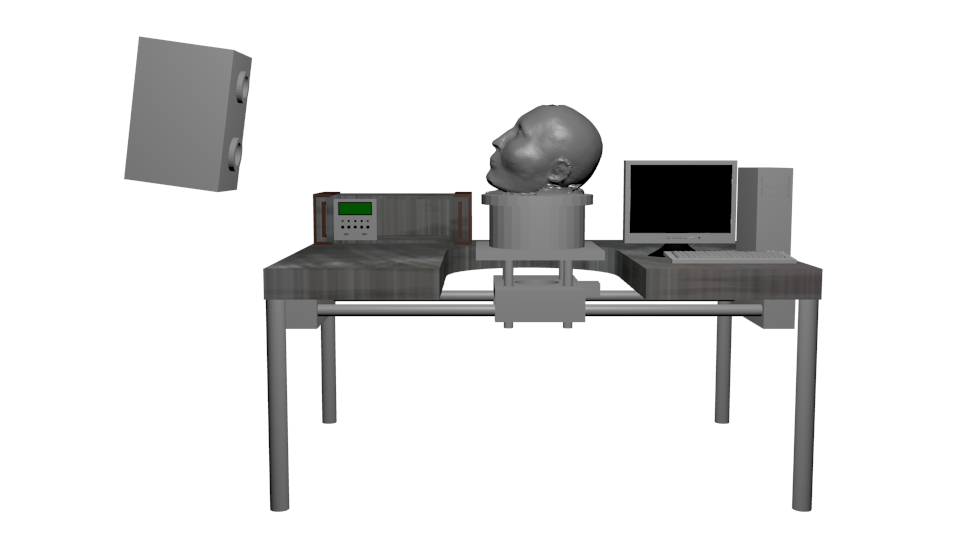
\includegraphics[width=\textwidth]{Blender/Schema_Arbeitsplatz.png}
\caption{Überblick des Arbeitsplatz}
\label{fig:Übersicht}
\end{figure}
\todo{ Komponenten auf Abbildung erwähnen!}

\section{Lasererfassungssystem VI-900}
\begin{figure}[htb]
\centering
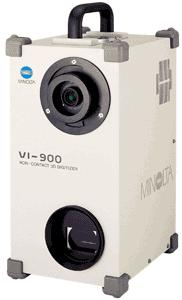
\includegraphics[width=100pt]{vi900-big.jpg}
\caption{VI-900}
\label{fig:VI900}
\end{figure}
Das Lasererfassungssystem \Fachbegriff{VI-900} der Firma \Fachbegriff{Minolta} besteht, wie auf Abbildung \ref{fig:VI900} zu sehen, aus einem \Fachbegriff{Lasertriangulator}(unten) und einer Kamera(oben). Das System lässt sich über eine \Fachbegriff{SCSI}-Schnittstelle ansprechen und konfigurieren. Zur mobilen Nutzung kann das Gerät auch auf der Rückseite bedient werden. Aufgenommene Daten können auf einer \Fachbegriff{CF-Karte} gespeichert werden. Im Projekt wurde jedoch lediglich die direkte Ansteuerung via SCSI genutzt.
\subsection{Lasertriangulator Prinzip}
Ein Lasertriangulator, wie in Abbildung \ref{fig:LaserTriangulator} zu sehen, besteht aus einem Laser, einem Linsensystem und im einfachsten Fall aus einer Pixeldetektorzeile. Der Laser strahlt auf ein Objekt und je nach Entfernung des Objektes wird das Streulicht unter einem anderen Winkel zurückgestrahlt. Das Streulicht wird durch die Linsen auf den Pixeldetektor abgebildet. Über die Position des Laserspots auf dem Pixeldetektor lässt sich auf die Entfernung des Objektes zurück schließen.\\
Der VI-900 digitalisiert Objekte durch ein Laser-Lichtschnittverfahren. Das vom Objekt reflektierte Licht wird von einer CCD-Flächenkamera erfasst, nach Ermittlung der Distanzwerte (Z-Achse) mittels Laser-Triangulation werden die 3D-Daten erstellt. Der Laserstrahl wird mit Hilfe eines hochpräzisen galvanischen Spiegels über das Objekt projiziert, pro Scan werden 640 x 480 Einzelpunkte erfasst.\cite{Minolta:Einleitung}\\
Die Technischen Daten befinden sich im Anhang in Tabelle \ref{tab:TD_VI-910}
\begin{figure}[htb]
\centering
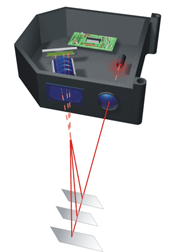
\includegraphics[width=100pt]{Laser-Triangulation.png}
\caption{Laser-Triangulation - Prinzip}
\label{fig:LaserTriangulator}
\end{figure}
\section{Ansteuerung für den Drehtisch}
Die Ansteuerung für den Drehtisch ist in einem 19*-Rack verbaut.
\begin{figure}[htb]
\centering
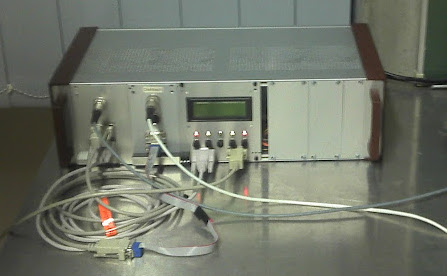
\includegraphics[width=100pt]{19Zoll_Rack}
\caption{Ansteuerung - 19''-Rack}
\label{fig:19Zoll_Rack}
\end{figure}
\subsection{Drehtisch}
\begin{figure}[htb]
\centering
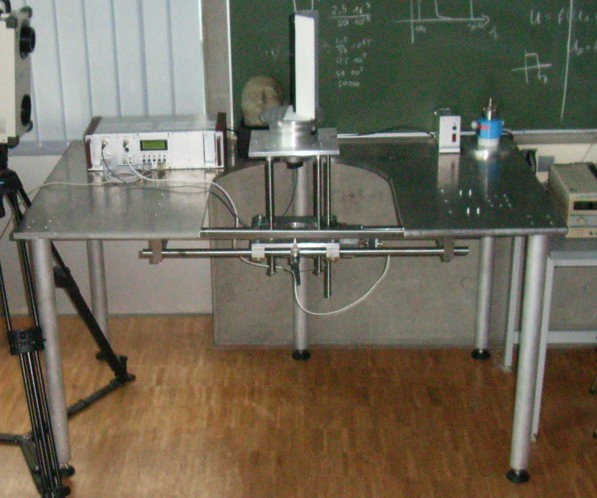
\includegraphics[width=100pt]{Drehtisch}
\caption{Drehtisch}
\label{fig:Drehtisch}
\end{figure}
Der Drehtisch(siehe Abbildung \ref{fig:Übersicht} ) ist eine Eigenkonstruktion der Werkstatt des RheinAhrCampus. Er besteht aus einer massiven Edelstahl Arbeitsplatte, welche auf 4 Füßen ruht. Aus dieser ist ein Rechteck mit aufgesetztem Halbkreis ausgeschnitten. In diesem Ausschnitt befindet sich der Drehtisch. Er ist auf einem Schienensystem gelagert. Mit dem Schienensystem kann der Drehtisch in der Vertikalen positioniert werden. Mit einem Schrittmotor lässt sich der Drehtisch sich zusätzlich in der Höhe verstellen. Die Höhenverstellung wird mit einem \Fachbegriff{Schneckengetriebe} realisiert. Ein weiterer Schrittmotor ist für die Drehung des Tisches zuständig. Der Tisch ist über ein \Fachbegriff{Harmonic-Drive-Getriebe} mit dem Schrittmotor verbunden. Das Übersetzungsverhältnis beträgt 1:50.   
\subsection{Spannungsversorgung}
Die Schrittmotorkarten werden von einem PC-Netzteil gespießt. Die Kabel waren direkt an die Verbindungsleisten gelötet. Um den Aufbau modular und erweiterbar zu machen, ersetzte ich die feste Lötverbindung durch eine Standard PC-Netzteil Verbindung. Dadurch kann das Netzteil nun einfach ausgebaut werden, bzw. das System leicht mit neuen Einschubkarten erweitert werden.\\
Die Logik der Schrittmotorkarten und die Mikrocontroller-Platine werden mit 5V gespeist. Zusätzlich wurden die Schrittmotorkarten mit 12V, für die die Schrittmotoren gespeist.
\begin{figure}[htb]
\centering
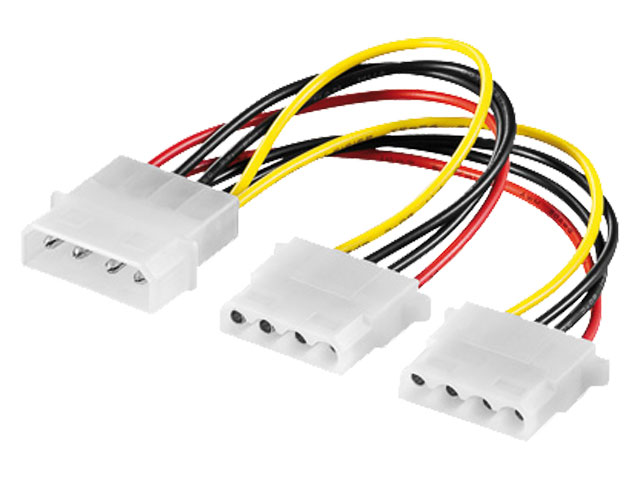
\includegraphics[width=100pt]{Y-Kabel.jpg}
\caption{Stromverbinder - Y-Kabel}
\label{fig:Y-Kabel}
\end{figure}
\todo{\url{http://www.kosatec.de/prod_images/kc/640x480/100539.jpg}}
\subsection{Schrittmotoren}
\todo{Motoren beschreiben! Technische Daten! Schritte, Spannungen. Verdrahtung.}

\subsection{Schrittmotorkarten}
Die Ansteuerung für die Schrittmotoren sind als 19"-Einschübe realisiert. Für jeden Schrittmotor wird ein Einschub benötigt.
Die Einschübe sind Produkte der Firma R+S. Mittels \Fachbegriff{RS-232 Schnittstelle} lassen sich die Karten konfigurieren und ansteuern. Die Konfiguration und Ansteuerung erfolgt über einen vorgegeben 
\Fachbegriff{ASCII}\footnote{Der American Standard Code for Information Interchange (ASCII, alternativ US-ASCII, oft [æski] ausgesprochen) ist eine 7-Bit-Zeichenkodierung\cite{wiki:ASCII}}
 Befehlssatz. Der Befehlssatz befindet sich im Kapitel \ref{sec:A_ASCII_Befehle}.Es können zwei oder mehr Karten als 
\Fachbegriff{Daisy-Chain}\footnote{Als Daisy Chain (englisch, wörtlich „Gänseblümchenkette“) bezeichnet man eine Anzahl von Hardware-Komponenten, welche in Serie miteinander verbunden sind (meist in sogenannten Bussystemen in der Automatisierungstechnik).\cite{wiki:Daisy} } 
in Reihe geschaltet werden.
\subsection{Motorverkabelung}
Die Schrittmotoren benötigen ein mindestens 4-adriges Kabel. Das Kabel für den Schrittmotor der für die Rotation zuständig ist war bereits gefertigt. Das Kabel für den Schrittmotor der für die Höhenverstellung zuständig ist, wurde selbst gefertigt. Hier wurden 3 weitere Adern für die beiden Endschalter benötigt.\\ Abbildung \ref{fig:Motorverkabelung} zeigt eine schematische Darstellung des Kabel. Tabelle \ref{tab:Motorverkabelung} gibt die Belegung der Kabel wieder.
\todo{Belegung überprüfen!}

\begin{figure}[htb]
\centering
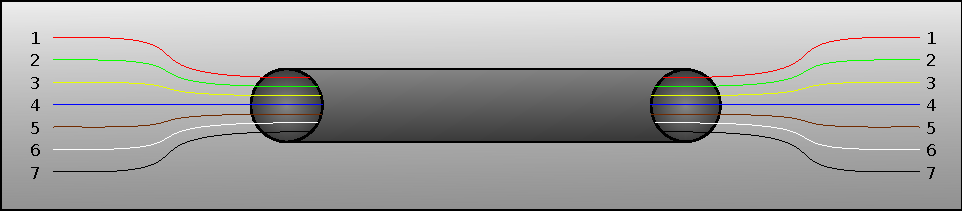
\includegraphics[width=\textwidth]{Kabel.pdf}
\caption{Motor- und Enschalterverkabelung}
\label{fig:Motorverkabelung}
\end{figure}


\begin{longtable}{|c|l|} 
\caption{Motor- und Endschalterverkabelung} \\
\hline
\label{tab:TD_VI-910}
1 & Phase A \\ 
\hline 
2 & Phase B \\ 
\hline 
3 & Phase C \\ 
\hline 
4 & Phase D \\ 
\hline 
5 & Endschalter Oben \\ 
\hline 
6 & Endschalter Unten \\ 
\hline 
7 & Endschalter Masse \\ 
\hline 
\end{longtable} 
\subsection{Endschalter}
Die Schrittmotorkarten unterstützen das Abschalten der Motoren wenn ein sogenannter Endschalter ausgelöst wird. Dies sind im allgemeinen mechanische Schalter die ausgelöst werden wenn der Tisch sich dem Ende des Arbeitsbereiches nähert. Dies verhindert eine Beschädigung des Aufbaus.\\
Im Aufbau waren bereits induktive Endschalter der Firma Pepperl+Fuchs verbaut. 
Normalerweise unterstützt die Schrittmotorkarte nur mechanische Endschalter. Durch geschickte Verdrahtung ließen sich die induktiven Endschalter verwenden. Hierzu musste über einen Spannungsteiler die Spannung herabgesetzt werden. Dadurch konnten die Endschalter direkt an die Optokoppler der Schrittmotorkarte angeschlossen werden. 
\begin{figure}[htb]
\centering
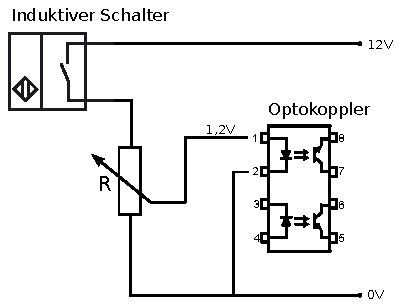
\includegraphics{Endschalter.pdf}
\caption{Motor- und Enschalterverkabelung}
\label{fig:Motorverkabelung}
\end{figure}\\
Am Drehtisch war ein Metallstutzen angebracht der den Endschalter auslösen sollte. Dieser war jedoch ungeeignet da er nicht dicht genug an den Induktiven Schalter heran kam, obwohl der Tisch schon in der Endposition war. Abhilfe schaffte ein längerer Metallstutzen der von der Werkstatt gefertigt wurde.\\
Wenn der Tisch sich in der Endposition befindet soll dies auch auf dem Mikrocontroller angezeigt werden. Die Signale der Endschalter liegen auf der Rückseite \todo{Zeichnung der Anschlüsse referenzieren.} am Verbindungsstecker an. Es muss also nur eine Brücke zu den entsprechenden Pins des Verbindungsstecker des Mikrocontroller gelötet werden.\\
Auf der Mikrocontroller Platine sind diese Pins mit zwei Pins des Mikrocontroller verbunden. Die beiden Pins werden im Mikrocontroller als Interrupts definiert. Die Interrupt-Service-Routine wird in Kapitel \ref{sec:Interrupts} beschrieben.

\section{Mikrocontroller}
Ein \Fachbegriff{Mikrocontroller} vereint, in einem IC, die wichtigsten Komponenten um komplexe technische Probleme leicht lösen zu können. Dazu gehören z.B. CPU, Flash-Speicher, Arbeitsspeicher, Register, Ports, ADC, DAC und mehr. Einen schematischen Überblick über die Komponenten eines Mikrocontroller bietet das Blockdiagramm in Abbildung \ref{fig:uC_Blockdiagramm}. \\
Um die Aufgaben zu lösen muss der Mikrocontroller mit einem Programm beschrieben werden. Diese Programme lassen sich am einfachsten in einer Entwicklungsumgebung, siehe Kapitel \ref{sec:Entwicklungsumgebung} schreiben. Diese Programme können dann z.B. Signale an Pins des Mikrocontroller auswerten und Signale über andere Pins wieder ausgeben und dadurch externe Geräte steuern. Eingehende Signale können binär ausgewertet werden oder mit einem ADC die Spannungshöhe bestimmt werden. Ausgehende Signale können auch binär oder mit einem DAC analog ausgegeben werden. Binäre Signale können zur Steuerung von LEDs oder Peripherie Geräten genutzt werden. Auch LC-Displays und Serielle Schnittstellen können so angesteuert werden.\\
Für unterschiedliche Aufgaben sind unterschiedliche Mikrocontroller geeignet. Zu Beginn stand ein ATmega 8515\cite{atmel:8515} im DIL-Gehäuse zur Verfügung. Dieser hatte 8 Kbyte Flash, 3 externe Interrupts, 1 Serielle Schnittstelle und konnte mit bis zu 16 MHz betrieben werden. 
Dieser war geeignet um sich in die Programmierung mit C ein zu finden und eine Serielle Schnittstelle an zu steuern. \\
Für dieses Projekt sind jedoch 2 externe Schnittstellen nötig. Der ATmega 324A\cite{atmel:324A} erfüllt diese Voraussetzung. Er ist dem ATmega 8515 recht ähnlich, bietet jedoch die benötigten 2 seriellen Schnittstellen. Des weiteren hat er 32 Kbyte Flash. Diese wurden aufgrund des recht umfangreichen Programms und den diversen Bibliotheken notwendig.
\begin{figure}[htb]
\centering
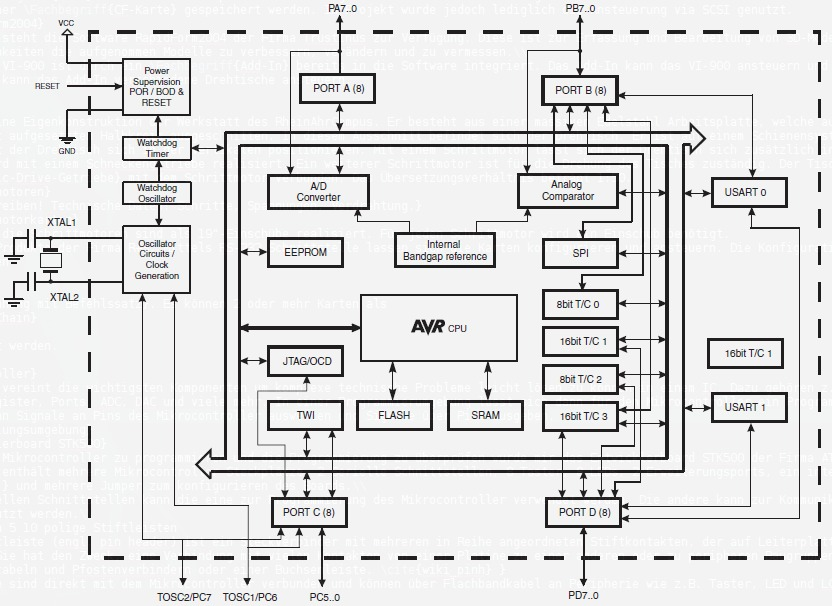
\includegraphics[width=\textwidth]{uC_Block}
\caption{Block Diagram eines Mikrocontroller}
\label{fig:uC_Blockdiagramm}
\citep{atmel:ug_324A}
\end{figure}
\subsection{Atmega 324A}
\todo{Blub}
\subsection{Entwicklerboard STK500}
Um Mikrocontroller zu programmieren und die Programmierung zu überprüfen kann das \Fachbegriff{Entwicklerboard} STK500(siehe Abbildung \ref{fig:STK500}) der Firma ATMEL verwendet werden. Das Board enthält mehrere Mikrocontroller Steckplätze, 2 Serielle Schnittstellen, 8 Taster, 8 LEDs, 2 Erweiterungsports, eine Programmierschnittstelle \Fachbegriff{ISP}\footnote{In System Programmer} und mehrere Jumper zum konfigurieren des Boards.\\
Von den beiden seriellen Schnittstellen kann die eine zur Programmierung des Mikrocontroller verwendet werden. Die andere kann zur Kommunikation mit dem Mikrocontroller genutzt werden.\\
Auf dem Board stehen fünf 10 polige Stiftleisten 
%\footnote{Eine Stiftleiste (engl. pin header) ist ein Steckverbinder mit mehreren in Reihe angeordneten Stiftkontakten, der auf Leiterplatten in der Elektronik Verwendung findet. Sie hat den Zweck, eine Verbindung mit vielen Kontakten von einer Platine zu einer anderen oder zu peripheren Baugruppen herzustellen, meist mit Hilfe von Flachbandkabeln und Pfostenverbindern oder einer Buchsenleiste. \cite{wiki:Stiftleiste} }
zur Verfügung. Diese sind direkt mit den Ports des Mikrocontroller verbunden und können über Flachbandkabel mit Peripherie wie z.B. Taster, LED, LC-Displays oder seriellen Schnittstellen verbunden werden.
\begin{figure}[htb]
\centering
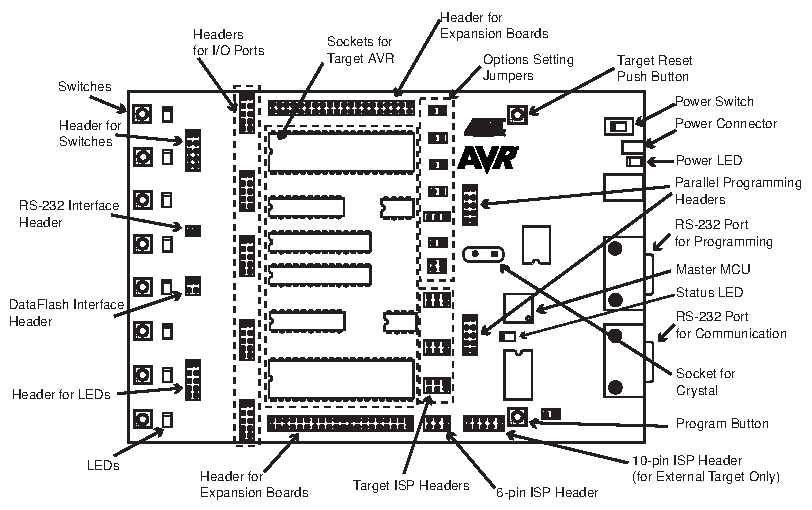
\includegraphics[width=\textwidth]{STK500_Schema.pdf}
\caption{Schema - STK500}
\label{fig:STK500}
\citep{atmel:ug_STK500}
\end{figure}

\subsection{AVRISP mkII}
Das AVRISP mkII ist ein USB-basiertes \Fachbegriff{In-System-Programmiersystem}. Dieses kann anstelle des RS-232 basierten Programmiersystem des STK500 verwendet werden.\\
Die Übertragungsgeschwindigkeit des AVRISP mkII ist wesentlich höher als die der Seriellen Schnittstelle. Desweiteren wurde der ATmega324A nicht mehr vom STK500 internen ISP unterstützt.\\
Der AVRISP mkII lässt sich einfach an den Programmierport, eine 6-Polige Stiftleiste, des STK500 anschließen.

\subsection{MAX232}
Die Spannungspegel des Mikrocontroller(typ. 0-5 V) sind nicht kompatibel zu den Spannungspegeln des RS-232 Standards (typ. -12-+12 V). Daher wird der \Fachbegriff{Pegelumsetzer} MAX232 genutzt. Dieser wandelt, mit internen Operationsverstärkern, die Spannungspegel auf für den RS-232 Standard passenden Wert.
\begin{figure}[htb]
\centering
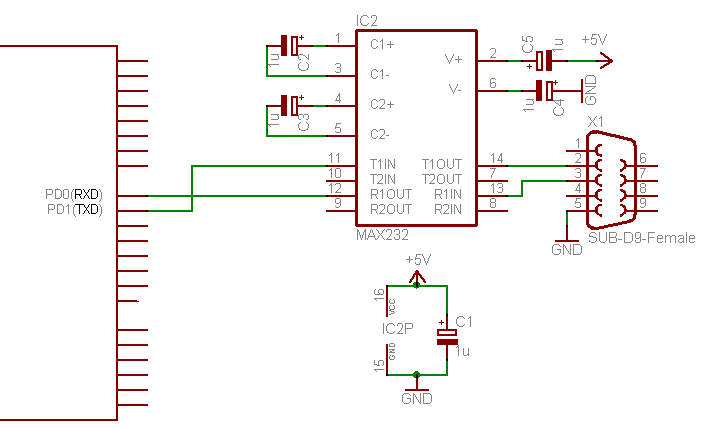
\includegraphics[width=0.6\textwidth]{AVR-RS232}
\caption{Schema - MAX232}
\label{fig:MAX232}
\citep{uC:RS232}
\end{figure}

\section{Platinenlayout}
Für den Mikrocontroller und seine Peripherie wurde ein Platinenlayout entwickelt. Dieses wurde in der Opensource Software KiCad entwickelt. \\ 
Dazu wurden die Schaltungen wie auf dem STK500 in den Schaltplan übernommen und dort das Layout entwickelt. 
\begin{figure}[htb]
\centering
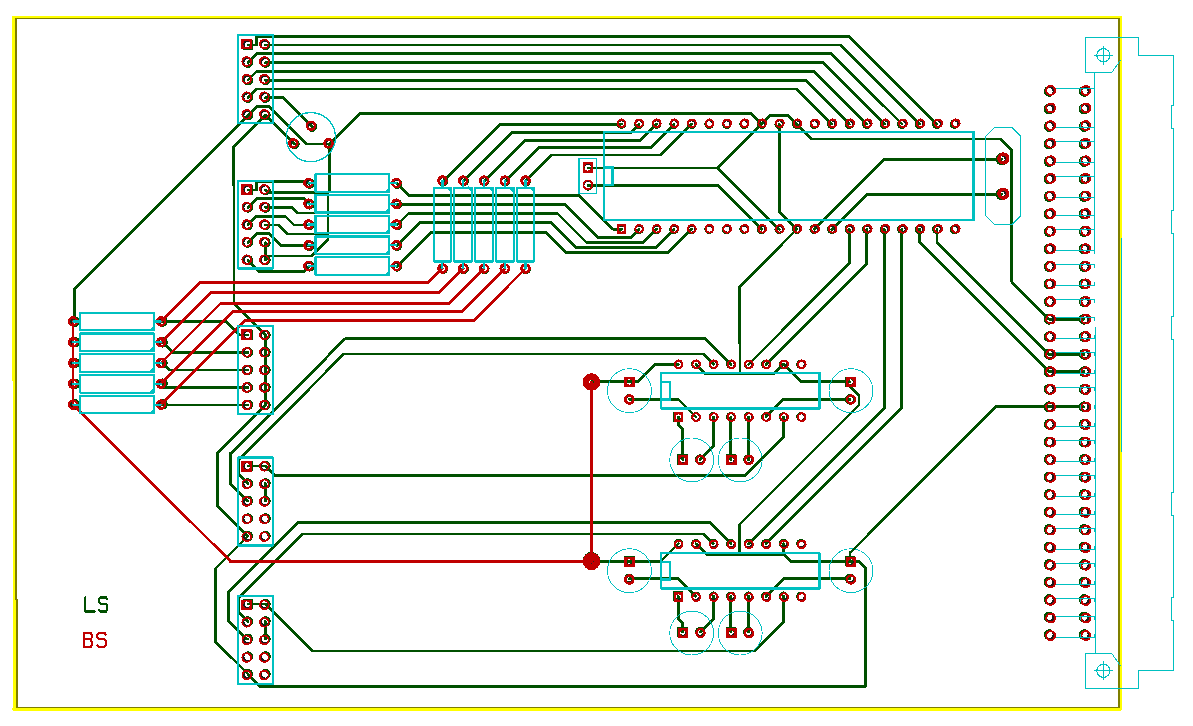
\includegraphics[width=\textwidth]{Translator_white}
\caption{Platinenlayout}
\label{fig:Platine}
\end{figure}
\todo{Schaltplan und einbinden.}
\section{19''-Einschub}
Die Platine für den Mikrocontroller wurde als 19"-Einschub konstruiert. Über den rückwärtigen Steckverbinden wird die Platine mit Spannung versorgt. Zusätzlich kommen hier auch die Signale der Endschalter an.
An der Vorderseite wird die Blende befestigt. Auf der Blende befinden sich das LC-Display, fünf Taster, 5 LEDs und 2 serielle Schnittstellen.\\ Alle Bauteile sind steckbar mit der Platine verbunden.